\label{sec:noisy_adders}
In this section, we are describing a noise model based on the assumption that the voltage to the actual circuit implementing the logic AND, OR or NOT gate is no longer kept constant resulting in variation of the {\em actual value} of the input to the AND, OR or NOT unit. We assume that the random variation is fully described through two parameters $\alpha \in \left[0,\frac{1}{2}\right]$ and $\beta \in \left[0,\frac{1}{2}\right]$ which denote the probability that a low-voltage input (i.e., bit state of $0$) switches to a high-voltage input (i.e., bit state of $1$) and vice versa\footnote{Note that a flip probability of more than 50\% means that the inverted gate would make less mistakes}. More formally, we assume that
\begin{align}
    P(a_\text{obs} = 1 | a = 0) & = \alpha\,, \label{eq:bit_flip_to_1} \\
    P(a_\text{obs} = 0 | a = 1) & = \beta\,. \label{eq:bit_flip_to_0}
\end{align}
With this noise model, it is possible that an AND, OR or NOT gate make mistakes in their computation. In the following table, we have listed the respective probability of each outcome $0$ and $1$ for the full list of bit-wise inputs $a$ and $b$.

\begin{center}
    \begin{tabular}{c|c||c|c||c|c||c|c}
        $a$                            & $b$                            &
        $P\left(a \land b = 0\right)$  & $P\left(a \land b = 1\right)$  &
        $P\left(a \lor b = 0\right)$   & $P\left(a \lor b = 1\right)$   &
        $P\left(\neg a = 0\right)$     & $P\left(\neg a = 1\right)$       \\
        \hline
        $0$                            & $0$                            &
        $1-\alpha^2$                   & $\alpha^2$                     &
        $\left(1-\alpha\right)^2$      & $1-\left(1-\alpha\right)^2$    &
        $\alpha$                       & $1-\alpha$                       \\
        $0$                            & $1$                            &
        $1-\alpha\left(1-\beta\right)$ & $\alpha\left(1-\beta\right)$   &
        $\left(1-\alpha\right)\beta$   & $1-\left(1-\alpha\right)\beta$ &
        $\alpha$                       & $1-\alpha$                       \\
        $1$                            & $0$                            &
        $1-\alpha\left(1-\beta\right)$ & $\alpha\left(1-\beta\right)$   &
        $\left(1-\alpha\right)\beta$   & $1-\left(1-\alpha\right)\beta$ &
        $1-\beta$                      & $\beta$                          \\
        $1$                            & $1$                            &
        $1-\left(1-\beta\right)^2$     & $\left(1-\beta\right)^2$       &
        $\beta^2$                      & $1-\beta^2$                    &
        $1-\beta$                      & $\beta$                          \\
    \end{tabular}
\end{center}
% \vspace{1em}

Note that this probability distribution reduces to point functions for $\alpha = \beta = 0$. Also, for $\alpha = \beta = \frac{1}{2}$, there is {\em still} information in the computation as the resulting probability distributions for AND and OR are not uniform.

\begin{figure}
    \begin{tabular}{ccc}
        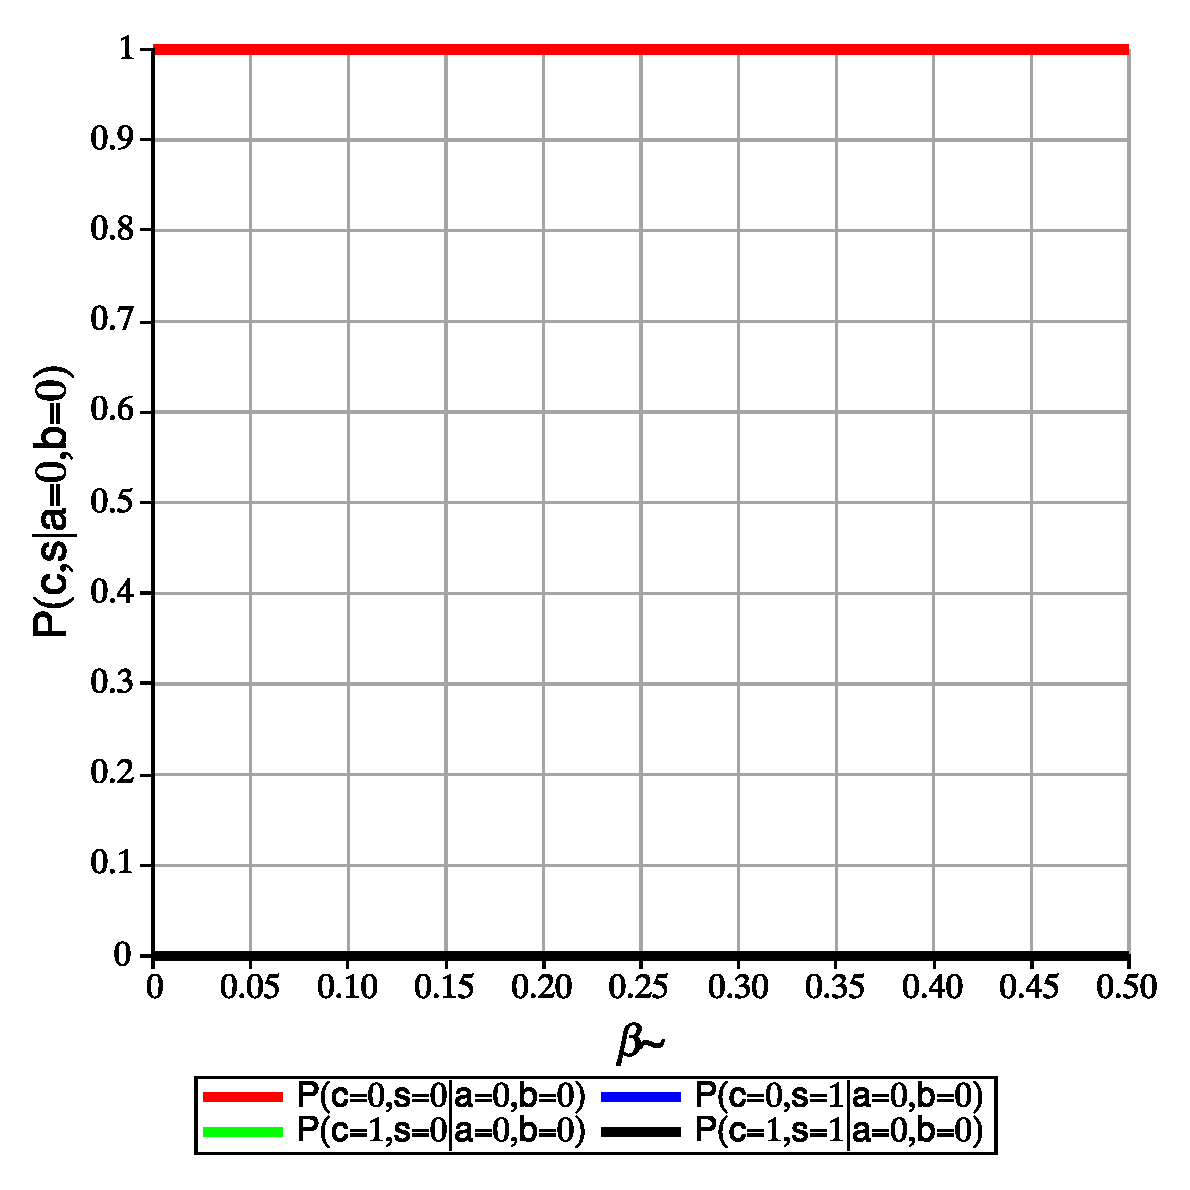
\includegraphics[width=.3\textwidth]{media/noisy_half_adder_value_dist_00.eps} &
        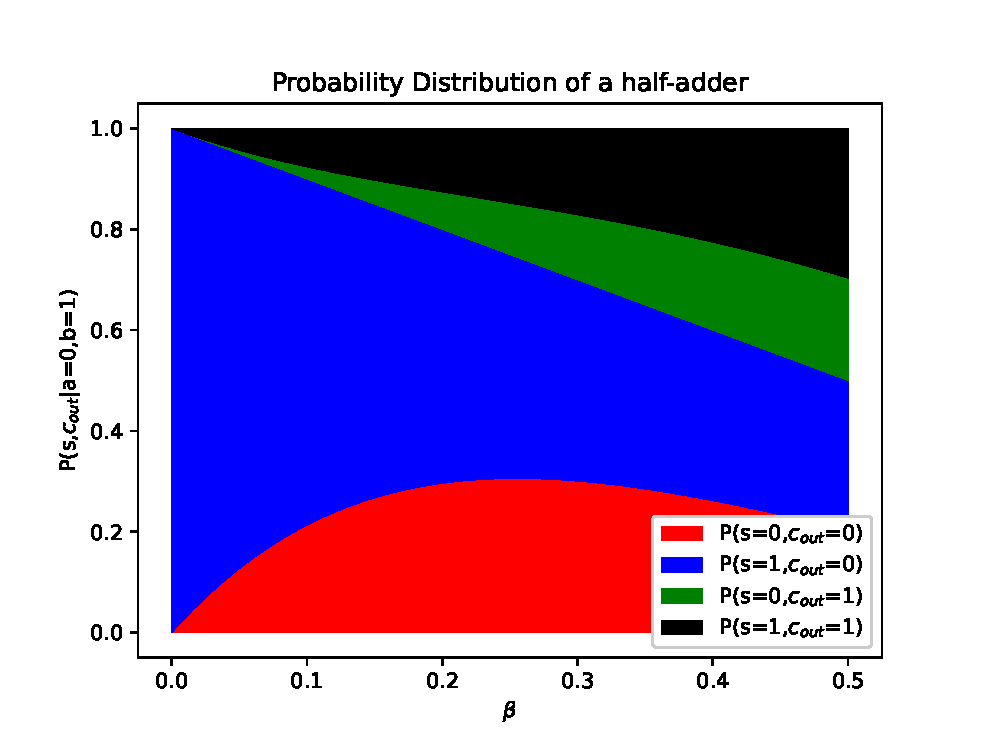
\includegraphics[width=.3\textwidth]{media/noisy_half_adder_value_dist_01.eps} &
        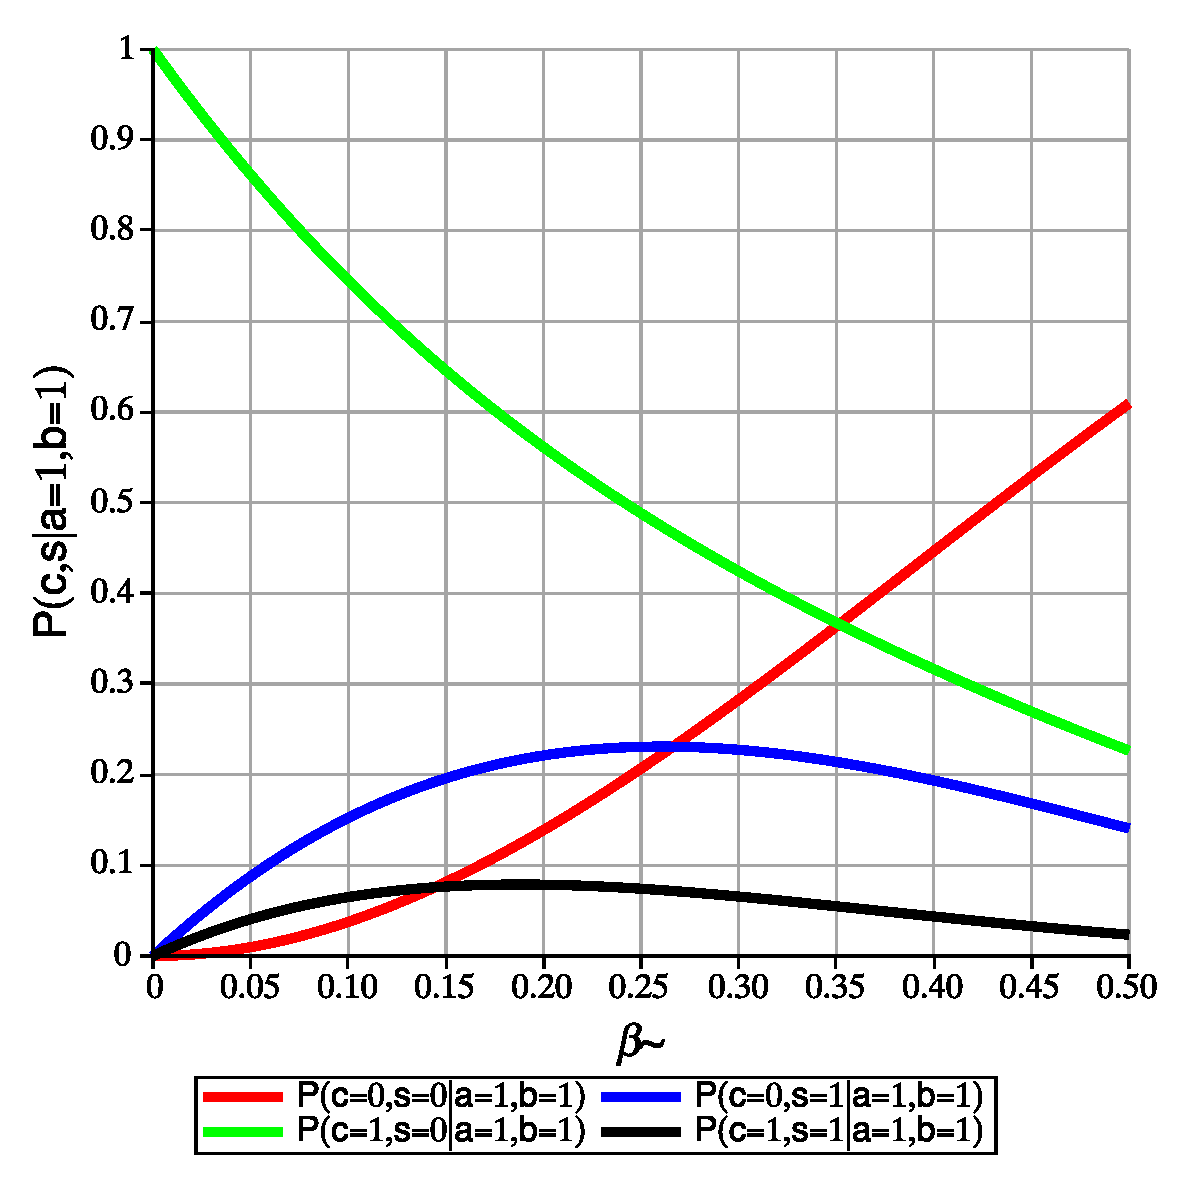
\includegraphics[width=.3\textwidth]{media/noisy_half_adder_value_dist_11.eps} 
    \end{tabular}
    \caption{Probability distribution for $P(s,c|a,b)$ for the three different cases of $a=0, b=0$ (left), $a=0, b=1$ (middle) and $a=1, b=1$ (right), respectively. The graphs show the change of the probability distributions as $\beta$ in (\ref{eq:bit_flip_to_0}) varies from $0$ to $\frac{1}{2}$ and $\alpha = 0$; this case is equivalent to assuming there is only leakage of information due to low-voltage. Note that the errors are not distributed based on the numerical distance of the results, e.g.\ for $\beta=40\%$ the sum of $a=b=1$ is $2$ with probability $\approx 30\%$, $1$ with probability $\approx 20\%$ but $0$ with probability $\approx 45\%$. \label{fig:noise_prob_dist}.}
\end{figure}

\paragraph{Noise Half Adders} Given the logic circuit design in the top row of Figure \ref{fig:half-and-full-adder}, we can now compute the marginal distribution over the sum bit $s$ and the carry-out bit $\cout$ of a half-adder by summing over all possible values of $d$ and $e$ using the probability distributions given above. More formally, we have 
\begin{align}
    P_\ha(s,\cout|a,b) & = \sum_{i=0}^1 \sum_{j=0}^1 P(s,\cout,d=i,e=j|a,b) \\
    & = \sum_{i=0}^1 \sum_{j=0}^1 P(\cout|a,b) P(d=i|a,b) P(e=j|\cout) P(s|d=i,e=j) \\
    & = P(\cout|a,b) \cdot \sum_{i=0}^1 \sum_{j=0}^1 P(e=j|\cout) P(d=i|a,b) P(s|d=i,e=j) \label{eq:noisy_half_adder} \,,
\end{align}
where the first line follows from the law of total probability, the second line follows from the directed graphical network structure $P(s,\cout,d,e|a,b)=P(\cout|a,b)P(d|a,b)P(e|\cout)P(s|d,e)$, and the third line follows from noticing that $P(\cout|a,b)$ does not depend on the value of $e$ and $d$. Note that even this simple model already results in a polynomial of degree 4 in both $\alpha$ and $\beta$. 

\paragraph{Noisy Full Adders} Using (\ref{eq:noisy_half_adder}) and the logic circuit design in the bottom row of Figure \ref{fig:half-and-full-adder}, we can now compute the marginal distribution over the sum bit $s$ and the carry-out bit $\cout$ of a full-adder by summing over all possible values of $d$, $e$ and $f$. We have 
\begin{align}
    P_\fa(s,\cout|a,b,\cin) & = \sum_{i=0}^1 \sum_{j=0}^1 \sum_{k=0}^1 P(s,\cout,d=i,e=j,f=k|a,b,\cin) \\
    & = \sum_{i=0}^1 \sum_{j=0}^1 \sum_{k=0}^1 P_\ha(d=i,e=j|a,b) P_\ha(s,f=k|\cin,d=i) P(\cout|e=j,f=k) \label{eq:noisy_full_adder} \,,
\end{align}
where the second line follows from the directed graphical network structure.

\paragraph{Noisy $4$-bit Adders} Finally, using (\ref{eq:noisy_half_adder}) and (\ref{eq:noisy_full_adder}), we can compute the marginal distribution over the output $S:=s_0s_1s_2s_3\cout^3$ of a $4$-bit adder of $A$ and $B$ by summing over all possible values of $\cout^0$, $\cout^1$ and $\cout^2$. We have 
\begin{align}
    P(S|A,B) & = \sum_{\cout^0=0}^1 \sum_{\cout^1=0}^1 \sum_{\cout^2=0}^1 P(s_0s_1s_2s_3\cout^3,\cout^0,\cout^1,\cout^2|A,B) \\
    & = \sum_{\cout^0=0}^1 \sum_{\cout^1=0}^1 \sum_{\cout^2=0}^1 P_\ha(s_0\cout^0|a_0,b_0)P_\fa(s_1\cout^1|a_1,b_1,\cout^0)\cdots P_\fa(s_3\cout^3|a_1,b_1,\cout^2)  \,,
\end{align}
where the second line follows from the directed graphical network structure.

In Figure \ref{fig:noise_prob_dist} we have shown how the resulting distributions vary as functions of $\alpha$ and $\beta$. One thing to note about this induced probability distribution is that for the case of $\alpha=0$ (i.e., it is not possible that any of the input bits ever flip erroneously from $0$ to $1$), the probabilities of a mistake of the noise half-adder for $a=0, b=0$ is zero for all values of $\beta$ but for either $a=0, b=1$ (or flipped) and $a=1, b=1$ there is probability that the $1$ input flips to zero resulting in an erroneous sum bit $s$ or carry bit $c$ (or both). In the next paragraph, we will present a solution attempt for this problem.



% \begin{figure}
%     \centering
%     \begin{tikzpicture}
%         % Circuit style
%         \ctikzset{
%             logic ports=ieee,
%             logic ports/scale=0.8,
%             % logic ports/fill=lightgray
%         }

%         % Logic ports
%         \node[or port] (OR) at (0,0){};
%         \node[and port] (ANDa1) at (0,-2){};
%         \node[and port] (ANDa2) at (0,-4){};
%         \node[or port] (OR2) at (2,-3){};
%         \node[not port] (NOT) at (4,-3){};
%         \node[and port] (ANDb) at (6,-1.5){};

%         % Input and output ports
%         \node (a) at (-2,-1) [left] {$a$};
%         \node (b) at (-2,-3) [left] {$b$};
%         \node (c) at (7,-4) [right] {$c$};
%         \node (c1) at (0.8,-2) [above] {$c_1$};
%         \node (c2) at (0.8,-4) [above] {$c_2$};
%         \node (d) at (1,0) [above] {$d$};
%         \node (e) at (4.8,-3) [above] {$e$};
%         \node (s) at (7,-1.5) [right] {$s$};
%         \node (af) [right = 0.5 of a, coordinate] [left] {};
%         \node (bf) [right = 1 of b, coordinate] [left] {};
%         \node (cf) at (3,-3) [coordinate] {};

%         % % Connection
%         \draw (ANDa1.out) -| (OR2.in 1);
%         \draw (ANDa2.out) -| (OR2.in 2);
%         \draw (OR2.out) -- (NOT.in);
%         \draw (OR.out) -| (ANDb.in 1);
%         \draw (NOT.out) -| (ANDb.in 2);

%         \draw (ANDb.out) -* (s);
%         \draw (OR.in 1) -| (af) |- (ANDa1.in 1);
%         \draw (OR.in 1) -| (af) |- (ANDa2.in 1);
%         \draw (OR.in 2) -| (bf) |- (ANDa2.in 2);
%         \draw (OR.in 2) -| (bf) |- (ANDa1.in 2);
%         \draw (a) -- (af);
%         \draw (b) -- (bf);
%         \draw (cf) |- (c);
%     \end{tikzpicture}
%     \caption{Logic circuit design of a half-adder function with carry-bit redundancy that computes the sum of two binary numbers $a \in \{0,1\}$ and $b \in \{0,1\}$ where $s$ is the sum of $a$ and $b$ and $c$ captures the carry-bit indicating an overflow (i.e., if $a$ and $b$ are both $1$, then $s=0$ and $c=1$). \label{fig:half-adder-fix-carry-bit-redundancy}}
% \end{figure}
